\documentclass[border=10pt]{standalone}
\usepackage{pgfplots}
\usepgfplotslibrary{colormaps}
\pgfplotsset{compat=1.18}

\begin{document}
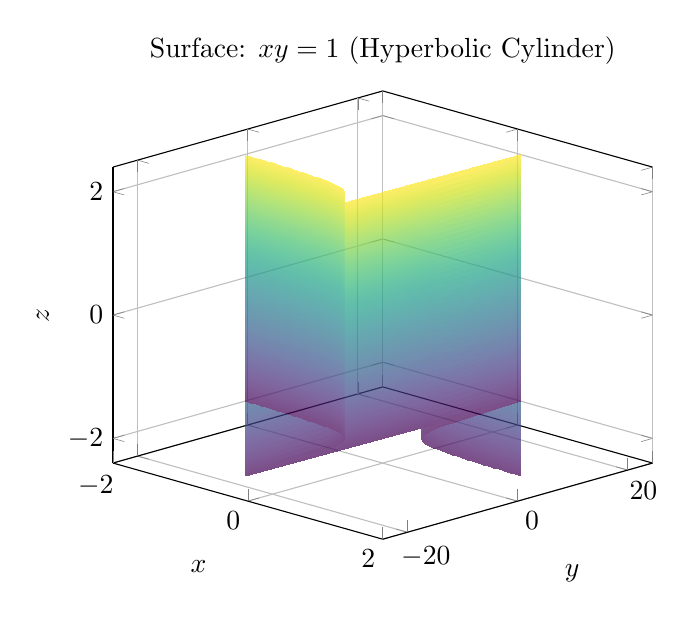
\begin{tikzpicture}
\begin{axis}[
    xlabel={$x$},
    ylabel={$y$},
    zlabel={$z$},
    title={Surface: $xy = 1$ (Hyperbolic Cylinder)},
    view={45}{20},
    colormap/viridis,
    grid=major,
    domain=-2:2,
    y domain=-2:2,
    samples=50,
    unbounded coords=jump,
    restrict z to domain=-2:2,
    ]
    \addplot3[surf, opacity=0.7, shader=interp] 
        ({x}, {1/x}, {y});
\end{axis}
\end{tikzpicture}
\end{document}